\documentclass[preprint,12pt]{elsarticle}
\usepackage{amsmath,amssymb,amsfonts}
\usepackage{algorithmic}
\usepackage{graphicx}
\usepackage{textcomp}
\usepackage{xcolor}
\usepackage{booktabs}
\usepackage{placeins}
\usepackage[colorlinks=true, linkcolor=black, citecolor=black, urlcolor=black]{hyperref}

\begin{document}

\begin{frontmatter}

\title{Fusion of CNN Models with Choquet Fuzzy Integral--Minkowski Distance--Parseval Theorem for Blood Cell Classification}

\author[inst1]{Debatra Banerjee}
\author[inst2]{Irina Shpakovskaya}
\author[inst3]{Olga Brikova}
\author[inst1]{Mahantapas Kundu}
\author[inst1]{Ram Sarkar}

\address[inst1]{Department of Computer Science and Engineering, Jadavpur University, Kolkata, India}
\address[inst2]{ENT Department, Pavlov First St. Petersburg State Medical University, Saint Petersburg, Russia}
\address[inst3]{Intelligent Devices Institute, Saint Petersburg Electrotechnical University ``LETI'', Saint Petersburg, Russia}

\begin{abstract}
This paper proposes a novel dual-branch deep learning architecture for automated blood cell classification that integrates local and global feature representations. The local branch employs a Gabor-filter-based CNN to capture fine-grained texture and orientation information, while the global branch incorporates shifted window multi-head self-attention to model long-range dependencies efficiently. To effectively combine these complementary features, a Choquet integral-inspired fuzzy fusion mechanism is introduced, enhanced by Minkowski distance for geometric divergence and Parseval-based energy alignment for uncertainty modeling. This fusion strategy enables adaptive, non-linear aggregation of features, improving robustness and discriminative capability. The proposed model is evaluated on BloodMNIST and WBC datasets, achieving high classification accuracy and outperforming several state-of-the-art methods. Extensive ablation studies demonstrate the effectiveness of each component, particularly the proposed fusion technique. The results highlight the potential of hybrid architectures with advanced fusion strategies for medical image classification tasks
\end{abstract}

\begin{keyword}
Blood Cell Classification \sep Gabor Filter \sep Shifted Window Attention \sep Choquet Integral \sep Minkowski Distance \sep Parseval Alignment
\end{keyword}

\end{frontmatter}

\FloatBarrier
\section{Introduction}
\subsection{Literature Survey}

Automated blood cell classification has attracted significant attention in medical image analysis due to its importance in diagnosing hematological disorders. With the advancement of deep learning, convolutional neural networks (CNNs) have become widely used for microscopic blood cell image classification. Fırat et al.~\cite{b23} proposed a multibranch lightweight CNN architecture incorporating an Inception module, pyramid pooling module (PPM), and depthwise squeeze-and-excitation block (DSEB) for peripheral blood cell classification. The proposed approach achieved high performance on multiple datasets including the BCCD, Raabin WBC, and PBC datasets, reporting accuracies of 99.96\%, 99.22\%, and 99.72\% respectively. Similarly, Girdhar et al.~\cite{b24} developed a CNN-based framework for white blood cell classification using the BCCD dataset, achieving an overall classification accuracy of 98.55\%.

In addition to blood cell classification, several studies in related medical imaging domains such as cervical cytology have demonstrated the effectiveness of advanced deep learning architectures. Payne et al.~\cite{b26} proposed a custom EfficientNet-based CNN model pre-trained on the MNIST dataset and fine-tuned for cervical cancer classification using LBC and SIPAKMED datasets. Their approach achieved accuracies of 97.14\% and 84.30\% respectively, highlighting the effectiveness of transfer learning for medical image classification tasks . Similarly, Sood et al.~\cite{b27} introduced a deep learning framework integrating transfer learning with attention mechanisms and preprocessing techniques such as Histogram of Oriented Gradients (HOG). Their method significantly improved classification performance, achieving up to 98.95\% accuracy using the Xception model on the Mendeley LBC dataset .

Further advancements have focused on hybrid and ensemble-based architectures to improve classification robustness and generalization. Singh et al.~\cite{b28} proposed a Modified High-Dimensional Feature Fusion (HDFF) framework that combines features from multiple pretrained CNN models including VGG16, ResNet50, DenseNet121, and Xception. The fused feature representation achieved up to 99.85\% accuracy across multiple datasets such as Herlev and SIPAKMED, demonstrating strong generalization and reduced misclassification rates . Similarly, Emon et al.~\cite{b29} introduced the MultiArchFusionV16Ensemble model, which integrates CNN, DNN, LSTM, and VGG16 architectures using a stacking ensemble approach. Their model achieved an accuracy of 98\% on the Mendeley LBC dataset, showing improved robustness and performance through architectural diversity . Additionally, Julie et al.~\cite{b30} proposed CervicalNet, a custom CNN-based computer-aided diagnostic system trained on the LBC dataset, achieving 97\% accuracy and demonstrating the feasibility of end-to-end deep learning models for automated classification .

Although CNN-based approaches have demonstrated strong performance, they often struggle to capture global contextual relationships due to their localized receptive fields. Consequently, effectively integrating both local structural details and long-range contextual dependencies remains a critical challenge in medical image classification. Motivated by these observations, this work explores a hybrid architecture that leverages complementary feature representations to improve classification performance on microscopic blood cell datasets.

\FloatBarrier
\subsection{Contributions}
In this paper, we have made the following contributions:
\begin{enumerate}
    \item\textbf{Gabor filter to capture local feature: } We have implemented gabor filter in a CNN to detect the local feature representation.
    \item\textbf{SWMHS attention to capture global feature: } We have implemented shifted window attention which is used in Swin transformer for analyzing the global dependencies with a CNN to reduce the complexity.
    \item\textbf{Fuzzy fusion: }Fuzzy logic here manifests through the implicit fuzzy measure $\mu$, where the joint measure $\mu(\{z_1, z_2\})$
    is not fixed but adapts based on feature interaction — becoming super-additive when branches are complementary and sub-additive when they conflict.  
\end{enumerate}



\FloatBarrier
\section{Methodology}

\FloatBarrier
\subsection{Proposed Architecture}

The input feature map is passed through two parallel branches at the same time. One branch consists of a customized convolutional neural network with one Gabor filter convolution layer which captures the fine orientations in the cells which acts as local branch. Another branch implements the windowed and shifted windowed multihead attention which is used in Swin transformer to capture the long range global dependencies. Then these outputs of two branches are fused using a novel Minkowski distance based Choquet integral fusion which gives a highly sophisticated, non-Euclidean decision boundary that adapts to the complex geometry of the feature space.

\FloatBarrier
\subsection{Gabor CNN Branch}

The Gabor filter is a Gaussian-modulated sinusoidal plane wave that provides optimal joint localization in both spatial and frequency domains. The gabor kernel for 2D input $(x,y)$ is given as
$$g(x, y; \lambda, \theta, \psi, \sigma, \gamma) = \exp\left(-\frac{x'^2 + \gamma^2 y'^2}{2\sigma^2}\right) \cdot \exp\left(i \left(2\pi \frac{x'}{\lambda} + \psi\right)\right)$$
with the rotated coordinates defined as
\[
\begin{aligned*}
x' &= x \cos\theta + y \sin\theta, \\
y' &= -x \sin\theta + y \cos\theta.
\end{aligned*}
\]

The Gabor kernel has two parts - the real part which is given by
$$g_{real}(x, y) = \exp\left(-\frac{x'^2 + \gamma^2 y'^2}{2\sigma^2}\right) \cos\left(2\pi \frac{x'}{\lambda} + \psi\right)$$
helps to detect ridge, responding maximally when a light line on a dark background or a dark line on a light background aligns with the center of the filter. 
and the imaginary part which is given by 
$$g_{imag}(x, y) = \exp\left(-\frac{x'^2 + \gamma^2 y'^2}{2\sigma^2}\right) \sin\left(2\pi \frac{x'}{\lambda} + \psi\right)$$
It acts as an edge detector, responding maximally to a step edge (a transition from dark to light) at the center of the filter.

The Gabor kernel function is controlled by 5 key parameters which are wavelength($\lambda$), orientation($\theta$), phase offset($\psi$), Gaussian envelope width($\sigma$) and spatial aspect ratio($\gamma$).

Now this Gabor kernel can be written in frequency domain which is also a Gaussian:
\[
G(u, v)
=
\exp\!\left(
- 2 \pi^2 \sigma^2
\left[
(u - f_0 \cos\theta)^2
+ \frac{(v - f_0 \sin\theta)^2}{\gamma^2}
\right]
\right)
\]
with the central frequency defined as
\[
f_0 = \frac{1}{\lambda}.
\]
In our Gabor CNN architecture there is one Gabor convolutional layer with 16 Gabor kernels. The Gabor kernel is applied on a 11x11 grid of the image. To apply the Gabor filter, we initialize our initial orientation, envelope width and wavelength randomly as 

$\theta_i \sim \mathcal{U}(0, \pi), \quad
 \sigma_i \sim \mathcal{U}(2, 5), \quad
 \lambda_i \sim \mathcal{U}(6, 10)$

Using this we compute the Gabor filter response, with 16 filters and $\theta_i \sim \mathcal{U}(0, \pi)$, the expected angular resolution is
$\Delta \theta_{avg} = \frac{\pi}{16} \approx 11.25^\circ$, which provides dense coverage of orientation space, enabling detection of edges at any angle.

After applying the Gabor filter on the input feature map we apply some subsequent layer. One ReLU activation is used for half-rectification of the input feature and introducing non-linearity into it. After this we apply 2D convolution, MaxPool, 2D convolution, MaxPool, AdaptiveAvgPool and at last flatten layer to generate the feature map. The final expression of the Gabor CNN can be written as

$\mathbf{f}_{local}
= \mathrm{GAP}(\mathrm{Pool}_2(\mathrm{ReLU}(\mathbf{W}_2 * \mathrm{Pool}_1(\mathrm{ReLU}(\mathbf{W}_1 * \mathrm{ReLU}(\mathbf{W}_{gabor} * \mathbf{X}))) + \mathbf{b}_2)))$

The orientation selectivity and frequency selectivity of Gabor filter helps to capture V1 simple cells, phase and position invariance of MaxPooling layer helps to capture V1 complex cells and the two deeper convolution layers help capture V2 and V4 cells(high visual areas).


\FloatBarrier
\subsection{CNN with shifted window attention}

While the Gabor branch provides exquisite sensitivity to local texture and edges, it lacks the ability to model long-range dependencies—the semantic relationship between pixels far apart in the image. Thats why to capture the global relationship we can apply a swin tranformer. swin is a hierarchical transformer which breaks the images into patches, finds a special type of shifted window multihead attention and then combines those patches. But swin is a quite heavyweight model, thats why we are using the shifted window mechanism with some CNN layers. 

In windowed multihead attention mechanism, we partition the input image into 7x7 non-overlapping patches(or windows) and self-attention is calculated for each window by the formula:
\[
\text{Attention}(Q, K, V) 
= \text{SoftMax}\left(\frac{QK^{T}}{\sqrt{d}} + B \right) V
\]

where $B$ is the relative position bias, a learnable parameter that encodes the relative spatial configuration of tokens within a window and
\begin{itemize}
\item $Q$ (Query): represents the feature vector of the current image patch (token) that is asking \emph{which other patches are relevant} to it.
\item $K$ (Key): represents the feature vectors of all candidate patches that describe \emph{what each patch contains}, used to match against the query.
\item $V$ (Value): represents the feature vectors carrying the \emph{actual information} of each patch that will be aggregated according to the attention weights.
\end{itemize}

Now windowed multihead attention has a very major drawback, windows are isolated so a window can not communicate with another window. So we device a shifted window attention. The window grid is shifted by (4,4) pixels towards the bottom right corner. There always remain an overlap which which acts as a bridge to propagate the information from one to another window. To implement the shifted window mechanism efficiently, we use a cyclic shift algorithm. The entire window is rolled i.e. shifted by 7 pixels up and left. 
A cyclic shift operation is applied using \texttt{torch.roll}.  
Let the feature map be a tensor $T \in \mathbb{R}^{H \times W}$.  
The shift operation is mathematically defined as:
\[
T_{\text{shifted}}(x, y)
=
T\!\left( (x + \text{shift}_x) \bmod W,\; (y + \text{shift}_y) \bmod H \right).
\]

The final feature map of CNN with shifted window attention

$\mathbf{f}_{global} = \mathrm{Proj}(\mathrm{GAP}(\mathrm{Pool}(\mathrm{SW\text{-}MSA}(\mathrm{W\text{-}MSA}(\mathbf{W}_{s2} * \mathrm{Pool}_1(\mathrm{ReLU}(\mathbf{W}_{s1} * \mathbf{X})))))))$


\FloatBarrier
\subsection{Fuzzy Fusion with Choquet Integral, Minkowski Distance, and Parseval Uncertainty}

\subsubsection{Feature Space Projection}

Given heterogeneous feature representations $\mathbf{f}_1 \in \mathbb{R}^{d_1}$ from the local branch and $\mathbf{f}_2 \in \mathbb{R}^{d_2}$ from the global branch (where $d_1 = 64$ and $d_2 = 256$), we first project them into a common semantic space $\mathbb{R}^d$ with $d = 128$ via learned linear transformations:
\begin{align*}
    \mathbf{z}_1 &= W_1 \mathbf{f}_1 + \mathbf{b}_1 \\
    \mathbf{z}_2 &= W_2 \mathbf{f}_2 + \mathbf{b}_2
\end{align*}
where $W_1 \in \mathbb{R}^{d \times d_1}$ and $W_2 \in \mathbb{R}^{d \times d_2}$ are the projection matrices, and $\mathbf{b}_1, \mathbf{b}_2 \in \mathbb{R}^d$ are the corresponding bias vectors.

\subsubsection{Classical Choquet Integral for Feature Fusion}

The Choquet integral provides a principled framework for aggregating multiple information sources under a non-additive fuzzy measure. Unlike weighted averaging, it captures synergistic and redundant interactions among feature sources, making it well-suited for multi-source information fusion.

Formally, let $U = \{z_1, z_2\}$ be the universe of discourse representing our two feature branches. A fuzzy measure $\mu: 2^U \rightarrow [0,1]$ assigns importance values to all subsets of $U$, satisfying:
\begin{align*}
    \mu(\emptyset) &= 0, \quad \mu(U) = 1 \\
    A \subseteq B &\implies \mu(A) \leq \mu(B) \quad \text{(monotonicity)}
\end{align*}

In our setting, Choquet aggregation is applied to the projected branch features $\mathbf{z}_1$ and $\mathbf{z}_2$ (not to the raw features $\mathbf{f}_1$ and $\mathbf{f}_2$). The classical Choquet integral of a non-negative feature scoring function $z: U \rightarrow \mathbb{R}^+$ with respect to a fuzzy measure $\mu$ is
\begin{equation*}
    \mathcal{C}_{\mu}(z) = \int z \, d\mu = \sum_{i=1}^{n} \bigl(z_{(i)} - z_{(i-1)}\bigr) \cdot \mu(A_{(i)}).
\end{equation*}
where $z_{(1)} \le z_{(2)} \le \cdots \le z_{(n)}$ denotes the sorted source contributions, $z_{(0)}=0$, and $A_{(i)}=\{(i),(i+1),\ldots,(n)\}$ is the suffix subset after sorting.

\paragraph{Feature Fusion under Classical Choquet.}
In the standard two-source setting with features $\mathbf{z}_1$ and $\mathbf{z}_2$, the Choquet integral collapses into a weighted combination governed by the individual and joint fuzzy measures: 

\begin{aligned*}
\mathbf{z}_{\text{fused}} 
&= \mu(\{z_1\}) \cdot \mathbf{z}_1 
  + \mu(\{z_2\}) \cdot \mathbf{z}_2  \\
&\quad + \Bigl[\mu(\{z_1, z_2\}) 
  - \mu(\{z_1\}) 
  - \mu(\{z_2\})\Bigr] 
  \cdot (\mathbf{z}_1 + \mathbf{z}_2)
\end{aligned*}

The key term $\mu(\{z_1, z_2\}) - \mu(\{z_1\}) - \mu(\{z_2\})$ captures the interaction:
\begin{itemize}
    \item \textbf{Super-additivity} ($\mu(\{z_1,z_2\}) > \mu(\{z_1\}) + \mu(\{z_2\})$): the features are complementary and reinforce each other.
    \item \textbf{Sub-additivity} ($\mu(\{z_1,z_2\}) < \mu(\{z_1\}) + \mu(\{z_2\})$): the features are redundant or conflicting.
\end{itemize}
This capacity for context-sensitive, non-linear aggregation is why the Choquet integral is preferred over simple weighted or concatenation-based fusion.

\paragraph{Limitations of Classical Choquet Fusion.}
Despite its theoretical appeal, the classical Choquet integral faces two fundamental challenges in practical multi-branch deep learning:

\begin{enumerate}
    \item \textbf{Absence of geometric divergence awareness.} When we want to use it for fusing different feature vectors, the classical formulation assigns fuzzy measures based on ordering of scalar importance scores, however, it does not explicitly account for the \emph{geometric discrepancy} between feature representations. Two branches may exhibit high individual energy  while being semantically divergent in feature space. Hence, with a distance-based modulation, the Choquet integral can distinguish between harmonious and conflicting feature pairs.

    \item \textbf{Lack of energy-consistent interaction modeling.} The joint fuzzy measure $\mu(\{z_1, z_2\})$ is typically hand-crafted or learned from data without explicitly encoding the \emph{shared semantic energy} between branches. As a result, alignment and uncertainty in feature correlation are not directly reflected in the fusion weights, leading to over- or under-reinforcement under ambiguous conditions.
\end{enumerate}

To address these limitations, we modify the Choquet integral framework with two complementary mechanisms: a \textit{Minkowski distance} for geometric divergence estimation, and a \textit{Parseval-based interaction coefficient} for energy-consistent uncertainty modeling. 

\subsubsection{Minkowski Distance for Geometric Divergence}

To overcome the first limitation, we introduce the Minkowski distance between the projected features $\mathbf{z}_1$ and $\mathbf{z}_2$ as an explicit measure of their geometric divergence. The general Minkowski distance of order $p$ is:
\begin{equation*}
    d_p(\mathbf{z}_1, \mathbf{z}_2) = \left( \sum_{i=1}^{d} |z_{1i} - z_{2i}|^p \right)^{1/p}
\end{equation*}

We adopt the Minkowski distance of order $p = 3$:
\begin{equation*}
    d_3(\mathbf{z}_1, \mathbf{z}_2) = \left( \sum_{i=1}^{d} |z_{1i} - z_{2i}|^3 \right)^{1/3}
\end{equation*}

The choice of $p=3$ is deliberate. Compared to the standard Euclidean distance ($p=2$), the cubic exponent assigns disproportionately higher penalty to large coordinate-wise deviations, making it more sensitive to strong feature discrepancies while remaining computationally tractable. This scalar quantity $d \in \mathbb{R}^+$ serves as an implicit fuzzy measure encoding the semantic agreement between the two branches:

\begin{itemize}
    \item \textbf{Low distance} ($d \rightarrow 0$): Feature representations exhibit high similarity, indicating potential redundancy.
    \item \textbf{Moderate distance} ($d \approx 1$): Feature representations capture complementary aspects of the input.
    \item \textbf{High distance} ($d \gg 1$): Feature representations are in semantic conflict, indicating potential noise or ambiguity.
\end{itemize}

The distance modulates the fusion through a normalization factor:
\begin{equation*}
    \alpha(d) = \frac{1}{1 + d_3(\mathbf{z}_1, \mathbf{z}_2)}
\end{equation*}
which satisfies the following mathematical properties: 
\begin{align*}
    \alpha(d) &\in (0, 1] \quad \forall \, d \geq 0 \quad \text{(bounded)} \\
    \frac{\partial \alpha}{\partial d} &= -\frac{1}{(1+d)^2} < 0 \quad \text{(monotonically decaying)} \\
    \lim_{d \to 0} \alpha(d) &= 1 \quad \text{(full reinforcement)} \\
    \lim_{d \to \infty} \alpha(d) &= 0 \quad \text{(complete suppression)}
\end{align*}

This ensures that when the two branches are geometrically close, their aggregation is fully reinforced, while strongly divergent representations are progressively suppressed.

\subsubsection{Parseval Inequality for Capturing Uncertainty in Alignment}

While the Minkowski distance captures geometric divergence, it primarily emphasizes point-wise deviations and does not explicitly encode the \emph{interaction strength} or shared semantic energy between features. Two feature vectors may exhibit small geometric distance while being weakly correlated, or conversely, show large distance while maintaining strong directional alignment . Therefore, a complementary mechanism is required to quantify feature-interaction under uncertainty, thereby addressing the second limitation of classical Choquet fusion.

To explicitly model semantic alignment and interaction strength, we adopt an energy-based formulation grounded in Parseval's identity and inequality. For a feature vector $\mathbf{z} \in \mathbb{R}^d$, Parseval's identity states that the total signal energy is:
\begin{equation*}
    \|\mathbf{z}\|_2^2 = \sum_{i=1}^{d} |z_i|^2
    \label{eq:parseval_identity}
\end{equation*}
This aggregates contributions across all dimensions, yielding a global and noise-robust measure of information content. Unlike distance metrics that focus solely on discrepancies, Parseval's identity directly characterizes the magnitude of the underlying representation, which is critical when feature reliability varies.

For two feature vectors $\mathbf{z}_1, \mathbf{z}_2 \in \mathbb{R}^d$, Parseval's inequality establishes an upper bound on their shared energy:
\begin{equation*}
    |\langle \mathbf{z}_1, \mathbf{z}_2 \rangle| \leq \|\mathbf{z}_1\|_2 \|\mathbf{z}_2\|_2
    \label{eq:parseval_inequality}
\end{equation*}
The inner product $\langle \mathbf{z}_1, \mathbf{z}_2 \rangle$ quantifies directional alignment and correlation between features, while the norms represent their respective energy magnitudes. This inequality guarantees numerical stability and ensures that interaction strength is governed by the uncertainty-aware energy of each feature source.

Based on this principle, we define a normalized energy interaction uncertainty coefficient:
\begin{equation*}
    \eta(\mathbf{z}_1, \mathbf{z}_2) = \frac{2\langle \mathbf{z}_1, \mathbf{z}_2 \rangle}{\|\mathbf{z}_1\|_2^2 + \|\mathbf{z}_2\|_2^2}, \quad \eta \in [-1, 1]
    \label{eq:eta}
\end{equation*}
This formulation is symmetric, scale-invariant, and explicitly accounts for both alignment and energy balance. Features with low energy (high uncertainty) naturally contribute less to the interaction, while strongly aligned high-energy features yield higher confidence scores. Unlike cosine similarity, this measure penalizes disproportionate energy contributions, which is desirable in fusion settings.

To ensure compatibility with fuzzy measure construction and Choquet integral-based aggregation, the interaction coefficient is mapped to the unit interval: 
\begin{equation*}
    A(\mathbf{z}_1, \mathbf{z}_2) = \frac{1 + \eta(\mathbf{z}_1, \mathbf{z}_2)}{2} \in [0, 1]
    \label{eq:alignment}
\end{equation*}
Here, $A(\mathbf{z}_1, \mathbf{z}_2)$ represents the degree of semantic agreement between the two feature sources: values close to 1 indicate strong alignment, values around 0.5 indicate neutral interaction, and values close to 0 indicate maximal disagreement.

\subsubsection{Implicit Fuzzy Measure Construction and Choquet-Inspired Fusion Operator}

The Minkowski distance and the Parseval-based interaction coefficient jointly define an implicit fuzzy measure over $U = \{z_1, z_2\}$, from which the final fusion operator is derived as a principled simplification of the full Choquet integral.

\paragraph{Defining implicit singleton fuzzy measure for each feature }
Each branch is assigned importance proportional to its Parseval energy:
\begin{align*}
    \mu(\{z_1\}) &= \frac{\|\mathbf{z}_1\|_2^2}{\|\mathbf{z}_1\|_2^2 + \|\mathbf{z}_2\|_2^2} \\[6pt]
    \mu(\{z_2\}) &= \frac{\|\mathbf{z}_2\|_2^2}{\|\mathbf{z}_1\|_2^2 + \|\mathbf{z}_2\|_2^2}
\end{align*}
Let $S = \|\mathbf{z}_1\|_2^2 + \|\mathbf{z}_2\|_2^2$. By construction, $\mu(\{z_1\}) + \mu(\{z_2\}) = S/S = 1$, so the two singletons form a \emph{partition of unity} — an additive baseline, where each branch contributes according to how much reliable signal it carries.

\paragraph{Defining joint implicit fuzzy measure }
\begin{equation*}
    \mu(\{z_1, z_2\}) \;=\; \mu(\{z_1\}) + \mu(\{z_2\}) + \frac{\eta(\mathbf{z}_1, \mathbf{z}_2)}{1 + d_3(\mathbf{z}_1, \mathbf{z}_2)}
\end{equation*}
The interaction term $\eta/(1{+}d_3)$ jointly encodes both dimensions of fusion quality: the \textbf{numerator} $\eta$ (Parseval) quantifies directional and energetic alignment, while the \textbf{denominator} $1+d_3$ (Minkowski) scales down the interaction as geometric divergence increases. This produces adaptive super/sub-additivity:
\begin{itemize}
    \item For small $d_3$ and positive interaction ($\eta > 0$): $\mu(\{z_1, z_2\}) > \mu(\{z_1\}) + \mu(\{z_2\})$, indicating \textbf{super-additivity} (complementarity).
    \item For large $d_3$ or negative interaction ($\eta < 0$): $\mu(\{z_1, z_2\}) < \mu(\{z_1\}) + \mu(\{z_2\})$, indicating \textbf{sub-additivity} (conflict or redundancy).
\end{itemize}

\paragraph{Derivation of the Fusion Operator with help of Choquet integral}
With the implicit fuzzy measure fully defined, we substitute it into the classical two-source Choquet formula to derive the fusion operator. According to Choquet integral, we can infer
\begin{equation*}
\begin{aligned}
    \mathbf{z}_{\text{fused}} = \,\, & \mu(\{z_1\}) \cdot \mathbf{z}_1 \\
    & + \mu(\{z_2\}) \cdot \mathbf{z}_2 \\
    & + \Bigl[ \mu(\{z_1, z_2\}) - \mu(\{z_1\}) - \mu(\{z_2\}) \Bigr] \cdot (\mathbf{z}_1 + \mathbf{z}_2)
\end{aligned}
\end{equation*}
 By substituting the coefficient of $z_1+z_2$ by we get
\begin{equation*}
\begin{aligned}
    \mu(\{z_1, z_2\}) - \mu(\{z_1\}) - \mu(\{z_2\}) &= \left[ 1 + \frac{\eta}{1+d_3} \right] - 1 \\
    &= \frac{\eta(\mathbf{z}_1, \mathbf{z}_2)}{1 + d_3(\mathbf{z}_1, \mathbf{z}_2)}
\end{aligned}
\end{equation*}
The singleton terms cancel exactly, leaving the interaction residual $\eta/(1+d_3)$ as the pure non-additive contribution.

Now substituting the singleton fuzzy parameters we get
\begin{equation*}
\begin{aligned}
    \mathbf{z}_{\text{fused}} = \,\, & 
        \frac{\|\mathbf{z}_1\|_2^2}{\|\mathbf{z}_1\|_2^2 + \|\mathbf{z}_2\|_2^2} \cdot \mathbf{z}_1 + 
        \frac{\|\mathbf{z}_2\|_2^2}{\|\mathbf{z}_1\|_2^2 + \|\mathbf{z}_2\|_2^2} \cdot \mathbf{z}_2
     \\
    & + 
        \frac{\eta(\mathbf{z}_1, \mathbf{z}_2)}{1 + d_3(\mathbf{z}_1, \mathbf{z}_2)} \cdot (\mathbf{z}_1 + \mathbf{z}_2)
\end{aligned}
\end{equation*}
This is the exact Choquet fusion under the implicit fuzzy measure, with no approximations applied yet.

In deep learning pipelines with batch normalization and shared projection dimensionality $d{=}128$, the projected features tend toward comparable energy magnitudes, i.e.\ $\|\mathbf{z}_1\|_2^2 \approx \|\mathbf{z}_2\|_2^2$, which implies $\mu(\{z_1\}) \approx \mu(\{z_2\}) \approx \tfrac{1}{2}$. The singleton terms then simplify to:
\begin{equation*}
    \frac{\|\mathbf{z}_1\|_2^2}{S}\cdot\mathbf{z}_1 + \frac{\|\mathbf{z}_2\|_2^2}{S}\cdot\mathbf{z}_2 \;\approx\; \tfrac{1}{2}(\mathbf{z}_1+\mathbf{z}_2) = \tfrac{1}{2}\,\mathbf{z}_{\text{sum}}
\end{equation*}
so the full expression becomes:
\begin{equation*}
    \mathbf{z}_{\text{fused}} \;\approx\; \left(\frac{1}{2} + \frac{\eta}{1+d_3}\right)\mathbf{z}_{\text{sum}}
\end{equation*}

The baseline $\tfrac{1}{2}$ above remains unmodulated by geometric compatibility. We impose that \emph{all} fusion — including the baseline — should be suppressed when geometric divergence is large, so we pull out $\alpha(d) = 1/(1+d_3)$ as a global multiplier:
\begin{align*}
    \mathbf{z}_{\text{fused}} &\;=\; \frac{1}{1+d_3}\!\left(\frac{1+d_3}{2} + \eta\right)\mathbf{z}_{\text{sum}} \\[6pt]
                               &\;\approx\; \frac{1}{1+d_3}\cdot\frac{1+\eta}{2}\cdot\mathbf{z}_{\text{sum}}
\end{align*}
Recognizing that $A(\mathbf{z}_1,\mathbf{z}_2) = (1+\eta)/2$ from Equation~\eqref{eq:alignment} and $\alpha(d) = 1/(1+d_3)$, we arrive at the compact form:
\begin{equation*}
\begin{aligned}
\mathbf{z}_{\text{fused}} 
&= \frac{A(\mathbf{z}_1,\mathbf{z}_2)}{1+d_3(\mathbf{z}_1,\mathbf{z}_2)}
   \cdot(\mathbf{z}_1+\mathbf{z}_2) \\[4pt]
&= A(\mathbf{z}_1,\mathbf{z}_2)\cdot\alpha(d)\cdot\mathbf{z}_{\text{sum}}
\end{aligned}
\end{equation*}

The three factors operate in cascade: $\mathbf{z}_{\text{sum}} = \mathbf{z}_1+\mathbf{z}_2$ carries the full combined feature response; $\alpha(d)$ suppresses geometrically conflicting pairs; and $A(\mathbf{z}_1,\mathbf{z}_2)$ further gates the result by directional and energetic coherence. Critically, both gating factors derive their values from the same implicit fuzzy measure — $\alpha(d)$ modulates the interaction term in $\mu(\{z_1,z_2\})$, and $A(\mathbf{z}_1,\mathbf{z}_2)$ is the Parseval-normalized form of $\eta$ — so $\mathbf{z}_{\text{fused}}$ is not an ad hoc formula but a mathematically derived collapse of the full Choquet integral under the energy-aware and distance-modulated fuzzy measure as constructed above. The complete pipeline is summarized in \autoref{tab:gabor_swin_algorithm}.

\begin{table}[h]
\centering
\caption{Operations in the Dual-Branch Gabor--Swin Fusion Network}
\label{tab:gabor_swin_algorithm}
\footnotesize
\setlength{\tabcolsep}{3pt}
\renewcommand{\arraystretch}{0.9}
\begin{tabular}{@{}ll@{}}
\toprule
\textbf{Step} & \textbf{Operation} \\
\midrule

Input & $\mathbf{X} \in \mathbb{R}^{B \times C \times H \times W}$ \\
Output & $\mathbf{y} \in \mathbb{R}^{B \times K}$ (class probabilities) \\

\midrule
\multicolumn{2}{l}{\textit{Local Feature Extraction (Gabor CNN Branch)}} \\

1. & Gabor Convolution: $\mathbf{G} \leftarrow \text{GaborConv}(\mathbf{X})$ \\

 & \quad $g(x,y)=\exp\!\left(-\frac{x'^2+\gamma^2y'^2}{2\sigma^2}\right)
      \exp\!\left(i(2\pi x'/\lambda+\psi)\right)$ \\

2. & Activation: $\mathbf{F}_1 \leftarrow \text{ReLU}(\mathbf{G})$ \\

3. & Conv Block: $\mathbf{F}_2 \leftarrow \text{Conv}_{3\times3}(\mathbf{F}_1)$ \\

4. & Pooling: $\mathbf{F}_3 \leftarrow \text{MaxPool}(\mathbf{F}_2)$ \\

5. & Conv Block: $\mathbf{F}_4 \leftarrow \text{Conv}_{3\times3}(\mathbf{F}_3)$ \\

6. & Pooling: $\mathbf{F}_5 \leftarrow \text{MaxPool}(\mathbf{F}_4)$ \\

7. & Global Pool: $\mathbf{f}_{local} = \text{GAP}(\mathbf{F}_5) \in \mathbb{R}^{B \times 64}$ \\

\midrule
\multicolumn{2}{l}{\textit{Global Feature Extraction (CNN + Shifted Window Attention)}} \\

8. & CNN Stem: $\mathbf{S}_1 \leftarrow \text{ReLU}(W_{s1} * \mathbf{X})$ \\

9. & Pool: $\mathbf{S}_2 \leftarrow \text{Pool}(\mathbf{S}_1)$ \\

10. & CNN Feature Map: $\mathbf{S}_3 \leftarrow W_{s2} * \mathbf{S}_2$ \\

11. & Window Attention: \\

 & \quad $\text{W-MSA}(Q,K,V) = \text{Softmax}\left(\frac{QK^T}{\sqrt{d}} + B\right)V$ \\

12. & Shifted Window Attention (cyclic shift): \\

 & \quad $T_{shift}(x,y) = T((x+s_x)\!\!\mod W,(y+s_y)\!\!\mod H)$ \\

13. & Global Pool: $\mathbf{f}_{global} = \text{GAP}(\mathbf{S}_3) \in \mathbb{R}^{B \times 256}$ \\

\midrule
\multicolumn{2}{l}{\textit{Feature Space Projection}} \\

14. & $\mathbf{z}_1 = W_1 \mathbf{f}_{local} + b_1 \in \mathbb{R}^{B \times 128}$ \\

15. & $\mathbf{z}_2 = W_2 \mathbf{f}_{global} + b_2 \in \mathbb{R}^{B \times 128}$ \\

\midrule
\multicolumn{2}{l}{\textit{Geometric Divergence Measurement}} \\

16. & Minkowski Distance $(p=3)$: \\

 & \quad $d_3(\mathbf{z}_1,\mathbf{z}_2) =
 \left(\sum_{i=1}^{d} |z_{1i}-z_{2i}|^3\right)^{1/3}$ \\

\midrule
\multicolumn{2}{l}{\textit{Energy-based Interaction (Parseval Formulation)}} \\

17. & Feature Energy: $\|\mathbf{z}\|_2^2 = \sum_i |z_i|^2$ \\

18. & Interaction Coefficient: \\

 & \quad $\eta(\mathbf{z}_1,\mathbf{z}_2) =
 \frac{2\langle \mathbf{z}_1,\mathbf{z}_2 \rangle}
 {\|\mathbf{z}_1\|_2^2 + \|\mathbf{z}_2\|_2^2}$ \\

19. & Agreement Score: \\

 & \quad $A(\mathbf{z}_1,\mathbf{z}_2) =
 \frac{1+\eta(\mathbf{z}_1,\mathbf{z}_2)}{2}$ \\

\midrule
\multicolumn{2}{l}{\textit{Choquet-Inspired Fusion}} \\

20. & Distance Normalization: $\alpha(d)=\frac{1}{1+d_3}$ \\

21. & Feature Aggregation: $\mathbf{z}_{sum}=\mathbf{z}_1+\mathbf{z}_2$ \\

22. & Fusion Operator: \\

 & \quad $\mathbf{z}_{fused}=A(\mathbf{z}_1,\mathbf{z}_2)\cdot
 \alpha(d_3)\cdot (\mathbf{z}_1+\mathbf{z}_2)$ \\

\midrule
\multicolumn{2}{l}{\textit{Classification}} \\

23. & Logits: $\mathbf{o} = W_{cls}\mathbf{z}_{fused} + b_{cls}$ \\

24. & Prediction: $\mathbf{y} = \text{Softmax}(\mathbf{o})$ \\

\bottomrule
\end{tabular}
\end{table}


\FloatBarrier
\section{Results and Discussion}

\FloatBarrier
\subsection{Software and Hardware Details}

Due to the lack of a dedicated GPU in our local machine, the entire model development and training process was carried out on the Kaggle platform using its cloud-based computational resources. We utilized two types of GPU accelerators provided by Kaggle: a dual-core NVIDIA Tesla T4 GPU, each core equipped with 16 GB GDDR6 VRAM, 2560 CUDA cores, and 320 Tensor Cores based on the Turing architecture; and a single-core NVIDIA Tesla P100 GPU with 16 GB HBM2 VRAM, 3584 CUDA cores, and no Tensor Cores, built on the Pascal architecture.

The model was implemented using the PyTorch deep learning library. Models are built using mainly PyTorch. Additional libraries such as Scikit-learn were used for dataset splitting and accuracy measurement; Matplotlib and Seaborn for visualization and data plotting; NumPy and Pandas for numerical and tabular data processing; and OpenCV for performing various preprocessing tasks.

\FloatBarrier
\subsection{Dataset Description}

Our model was primarily evaluated using the BloodMNIST dataset to perform eight-class classification of breast cancer stages. This dataset contains $28x28$ images of various type of blood cells. The 8 classes available in BloodMNIST dataset are namely basophil, eosinophil, erythroblast, immature granulocytes, lymphocyte, monocyte ,neutrophil, platelet The original dataset contains microscopic images of blood cells colored with May Grünwald-Giemsa stain. The images are 363x363 firstly, then they are centre-cropped to 200x200 images and resized to 28x28. BloodMNIST dataset is one of the many standard medical dataset under the MedMNIST. The whole dataset contains 17,092 images which are divided into a 70\%-10\%-20\% ratio, totaling 11,959 training, 1,712 validation, and 3,421 test samples.

We also implemented our model on a dataset named White Blood Cells dataset. This dataset is available in Kaggle. This dataset contains a train set of 10,265 images and 2 test sets i.e Test A and Test B where Test A contains samples for multiclass classification with class names as Basophil, Eosinophil, Lymphocyte, Monocyte, Neutrophil same as the training set and Test B contains samples for binary classification with class names as Lymphocyte and Neutrophil. We are only using our model for the multiclass classification dataset. 

\FloatBarrier
\subsection{Hyperparameters}

The proposed dual-branch architecture, consisting of a Gabor-based convolutional local branch and a manually implemented Swin Transformer like CNN for global feature extraction, was trained from scratch without the use of pretrained weights. Model optimization was performed using the Adam optimizer with an initial learning rate of $1\times10^{-4}$. The default Adam momentum parameters were used, with $\beta_1 = 0.9$, $\beta_2 = 0.999$, and $\epsilon = 1\times10^{-8}$, and the AMSGrad variant was not employed. The network was trained for a total of 25 epochs using a batch size of 16. To ensure reproducibility, a fixed random seed of 42 was used for all experiments. Training was conducted on a GPU when available; otherwise, CPU execution was used.

For supervision, the standard categorical cross-entropy loss (\texttt{CrossEntropyLoss}) with mean reduction was employed, without the use of class weights, label smoothing, or ignore index modifications. No explicit learning rate scheduler or early stopping strategy was applied, and the learning rate remained fixed throughout the training process. Regularization was implicitly introduced through data augmentation, including random horizontal flipping and random rotations up to $10^\circ$ applied to the training images. The DataLoader was configured with shuffling enabled for the training set to encourage better generalization, while shuffling was disabled for both validation and test sets to ensure consistent and deterministic evaluation. Model performance was assessed using classification accuracy, class-wise precision, recall, and F1-score, along with confusion matrix analysis on the held-out test set.

The computational cost of the proposed architecture arises from the combination of a lightweight Gabor-based convolutional local branch and a manually implemented Swin Transformer CNN for global representation learning. The local branch consists of a single Gabor convolution followed by shallow convolutional layers and global average pooling, resulting in a relatively low computational overhead proportional to $\mathcal{O}(HWk^2C)$, where $H$ and $W$ denote the spatial dimensions, $k$ is the kernel size, and $C$ is the number of channels. In contrast, the global branch dominates the overall complexity due to the multi-stage transformer encoder. The self-attention mechanism in each Swin block incurs a computational cost of $\mathcal{O}(N \cdot d^2)$ per block, where $N$ is the number of patch tokens and $d$ is the embedding dimension, while patch merging progressively reduces the token count across stages to control complexity.

Training was performed end-to-end from scratch without parameter freezing or pretrained initialization. With an input resolution of $224 \times 224$ and a batch size of 16, the model converged within 25 epochs. On a single GPU, each training epoch required several minutes depending on hardware availability, while CPU-based training incurred a significantly higher runtime. Despite the absence of window-shifted attention and pretrained weights, the architecture remained computationally feasible due to aggressive patch downsampling and dimensionality reduction in later Swin stages. During inference, the model processes each image in a single forward pass, making it suitable for offline medical image analysis scenarios where accuracy is prioritized over real-time constraints.



\FloatBarrier
\subsection{Results}

For the BloodMNIST dataset, we have achieved 98.32\% training accuracy with .0123 training loss, 97.98\% validation accuracy with 0.0138 validation loss. The test metrics are shown in \autoref{tab:breakhis_metrics}. The confusion matrix is shown in \autoref{fig:breakhis_confusion}.


\begin{table}[h!]
\centering
\caption{Results obtained on the BloodMNIST dataset}
\label{tab:breakhis_metrics}
\begin{tabular}{lcccc}
\hline
\textbf{Class} & \textbf{Precision} & \textbf{Recall} & \textbf{F1-score} & \textbf{Support} \\
\hline
basophil                & 1.0000 & 1.0000 & 1.0000 & 1.0000 \\
eosinophil       & 0.9748 & 0.9721 & 0.9696 & 0.9712 \\
erythroblast      & 0.9521 & 0.9595 & 0.9404 & 0.9595 \\
immature\_granulocytes     & 0.9484 & 0.9566 & 0.9571 & 0.9492 \\
lymphocyte    & 0.9799 & 0.9865 & 0.9832 & 0.9865 \\
monocyte         & 0.9866 & 0.9932 & 0.9899 & 0.9932 \\
neutrophil     & 0.9933 & 1.0000 & 0.9966 & 1.0000 \\
platelet    & 1.0000 & 1.0000 & 1.0000 & 1.0000 \\
\hline
\textbf{Average}   & 0.9707 & 0.9796 & 0.9721 & 0.9733 \\
\hline
\end{tabular}
\end{table}

\begin{figure}[!ht]
    \centering
    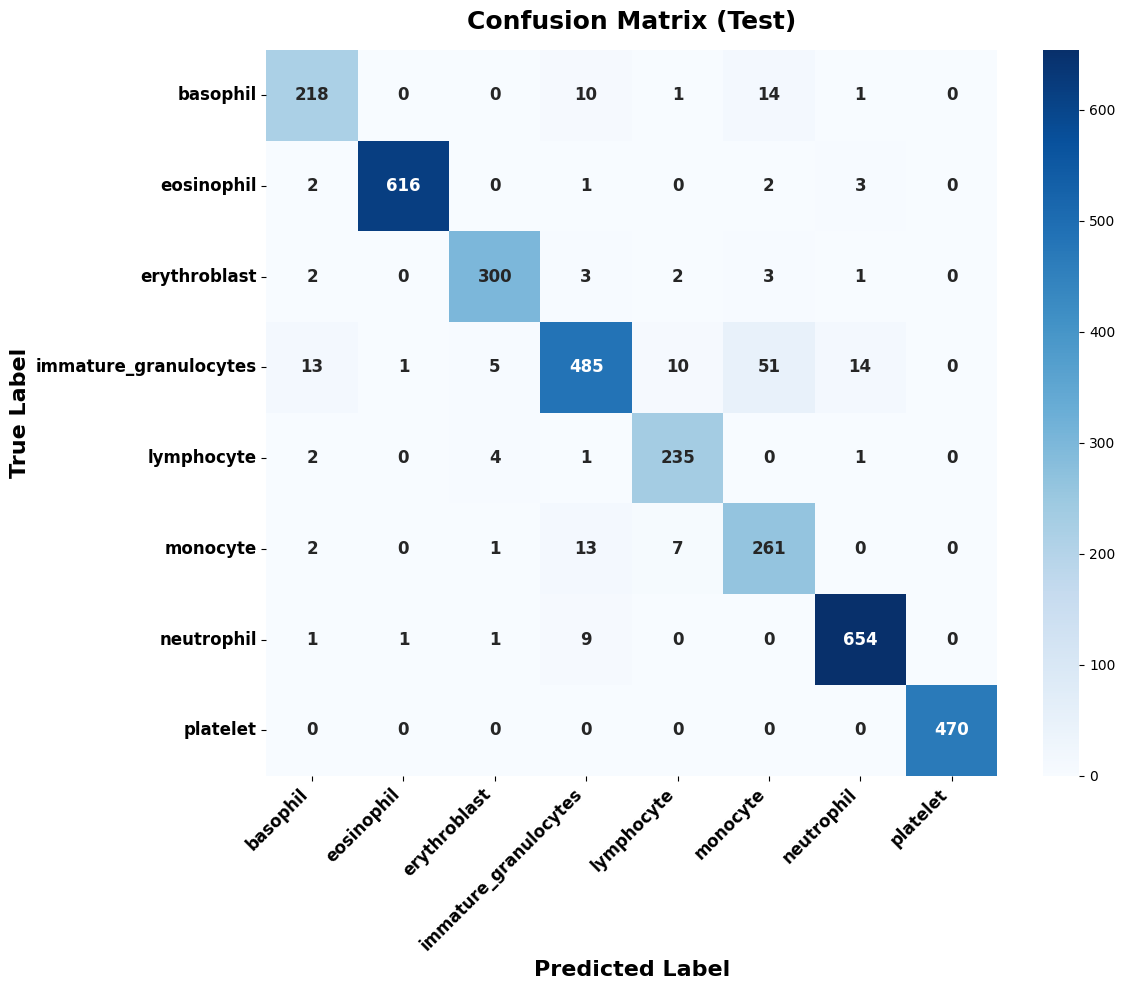
\includegraphics[width=0.7\linewidth]{confusion matrix1.png} 
    \caption{Confusion matrix on the BloodMNIST dataset. }
    \label{fig:breakhis_confusion}
\end{figure} 

For the WBC dataset, we have achieved 99.67\% training accuracy with .0082 training loss and 98.86\% validation accuracy with .0212 validation loss. The test scores are shown in \autoref{tab:bach_metrics}. The confusion matrix is shown in \autoref{fig:bach_confusion}. Feature-space separability analysis using t-SNE is presented in \autoref{tab:tsne_results}, and class-discriminative attention behavior from Grad-CAM is shown in \autoref{tab:gradcam_results}.
\begin{table}[h!]
\centering
\caption{Results on the WBC dataset}
\label{tab:bach_metrics}
\begin{tabular}{lcccc}
\hline
\textbf{Class} & \textbf{Precision} & \textbf{Recall} & \textbf{F1-score} & \textbf{Accuracy} \\
\hline
Basophil      & 0.9888 & 0.9897 & 0.9852 & 0.9869 \\
Eosinophil      & 0.9806 & 0.9801 & 0.9809 & 0.9807 \\
Lymphocyte      & 0.9412 & 0.9410 & 0.9409 & 0.9405 \\
Monocyte    & 0.9511 & 0.9515 & 0.9510 & 0.9530 \\
Neutrophil      & 0.9543 & 0.9541 & 0.9531 & 0.9533 \\ 
\hline
\textbf{Average}       & 0.9531 & 0.9542 & 0.9541 & 0.9550 \\
\hline
\end{tabular}
\end{table}




\begin{figure}[!ht]
    \centering
    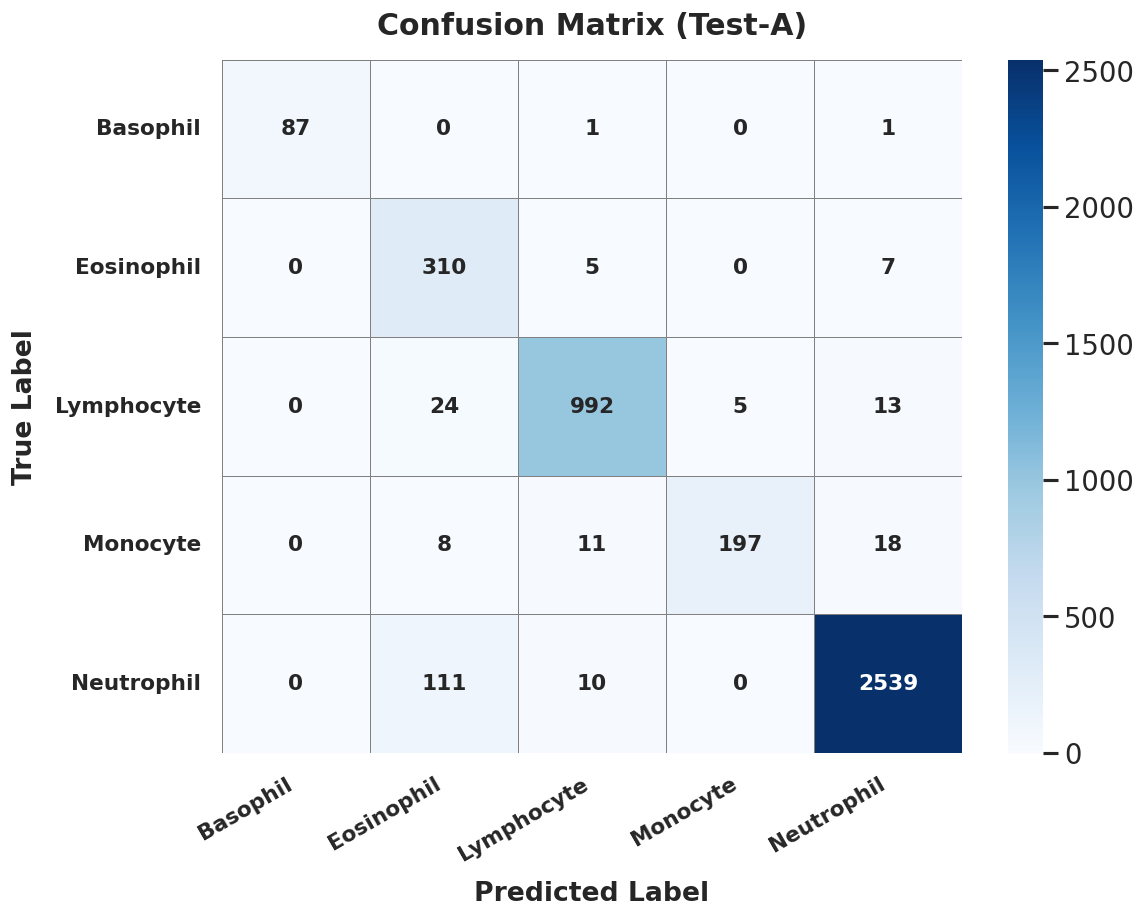
\includegraphics[width=0.7\linewidth]{confusion matrix3.png} 
    \caption{Confusion matrix of the WBC dataset. }
    \label{fig:bach_confusion}
\end{figure} 


\begin{table*}[t]
\centering

% �� Spacing improvements
\renewcommand{\arraystretch}{1.5}
\setlength{\tabcolsep}{8pt}

\resizebox{\linewidth}{!}{%
\begin{tabular}{|c|c|c|}
\hline

% ===================== BloodMNIST =====================
\multicolumn{3}{|c|}{\LARGE \textbf{BloodMNIST}} \\[8pt] \hline

\begin{tabular}{c}
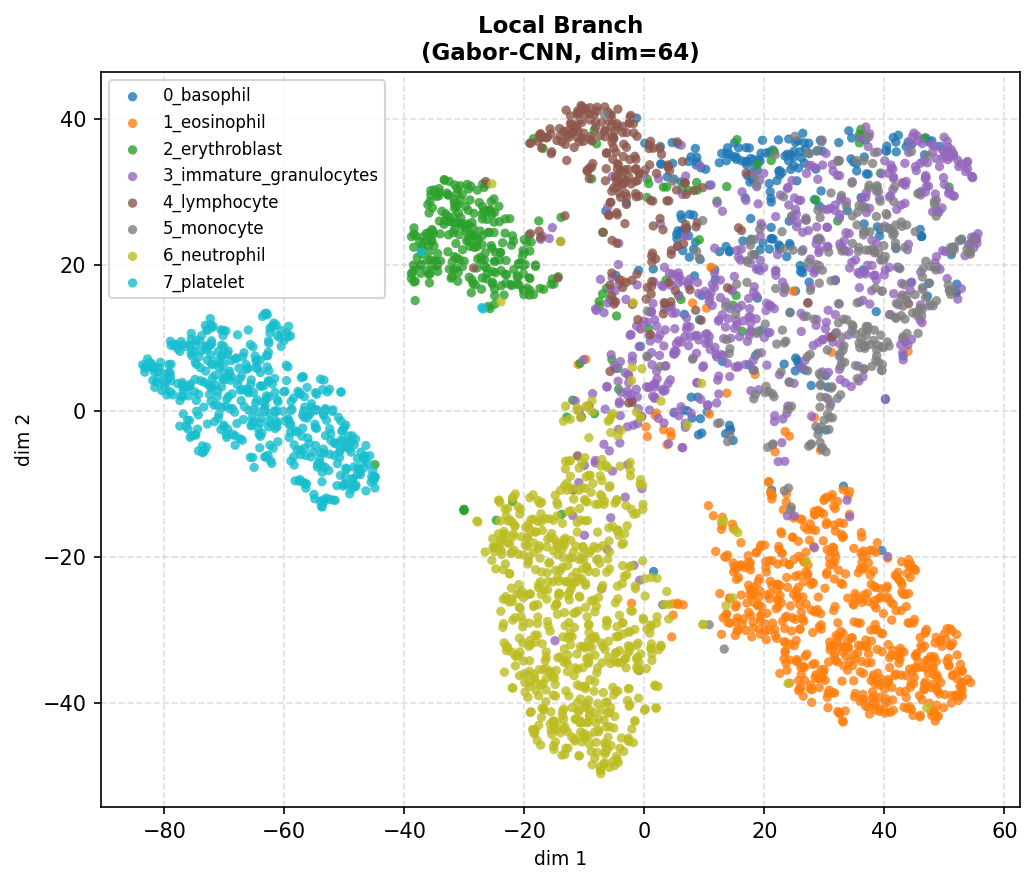
\includegraphics[width=0.5\linewidth]{tsne_local_branch (1).png} \\
\textbf{(a)}
\end{tabular}
&
\begin{tabular}{c}
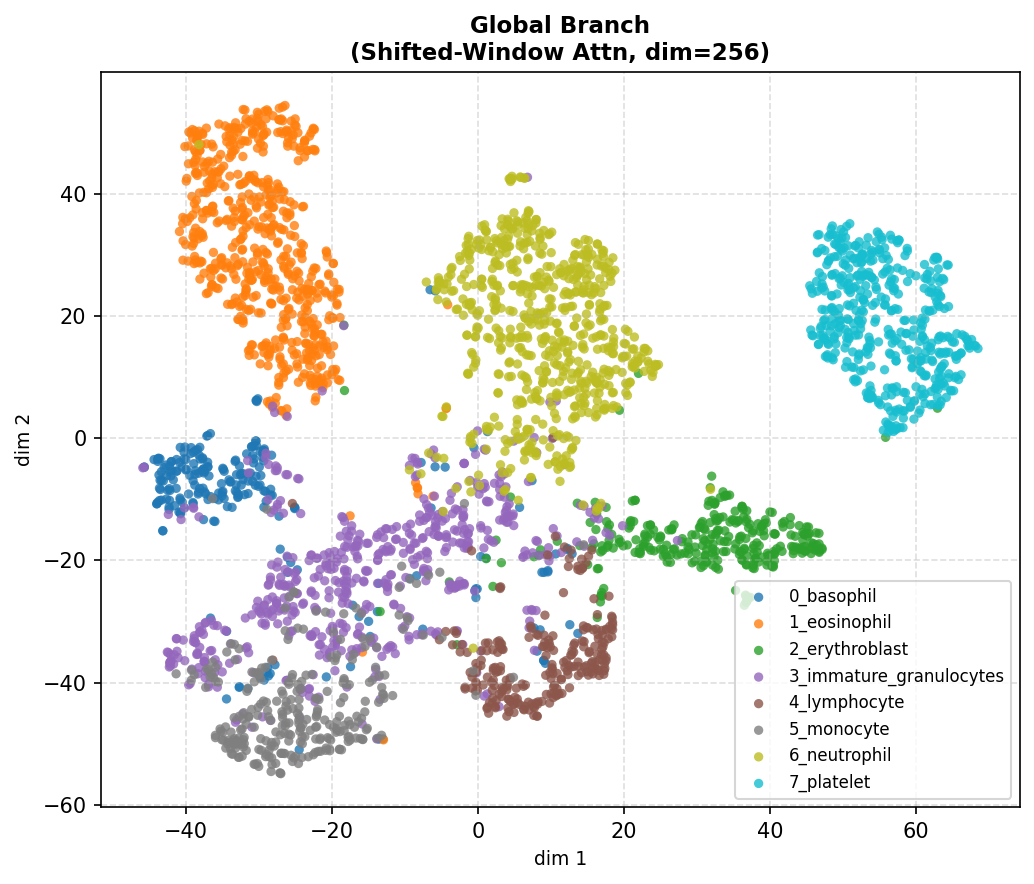
\includegraphics[width=0.5\linewidth]{tsne_global_branch (1).png} \\
\textbf{(b)}
\end{tabular}
&
\begin{tabular}{c}
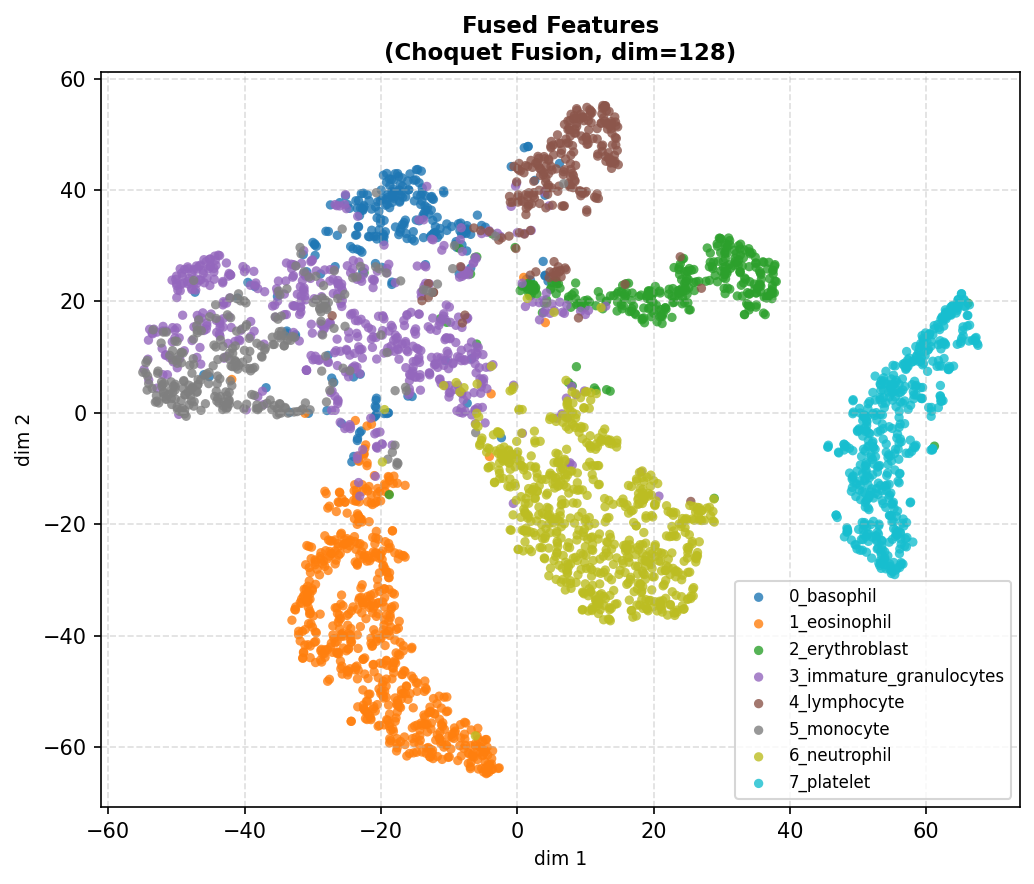
\includegraphics[width=0.5\linewidth]{tsne_fused (1).png} \\
\textbf{(c) Fusion}
\end{tabular}
\\ \hline

% ===================== WBC =====================
\multicolumn{3}{|c|}{\LARGE \textbf{WBC}} \\[8pt] \hline

\begin{tabular}{c}
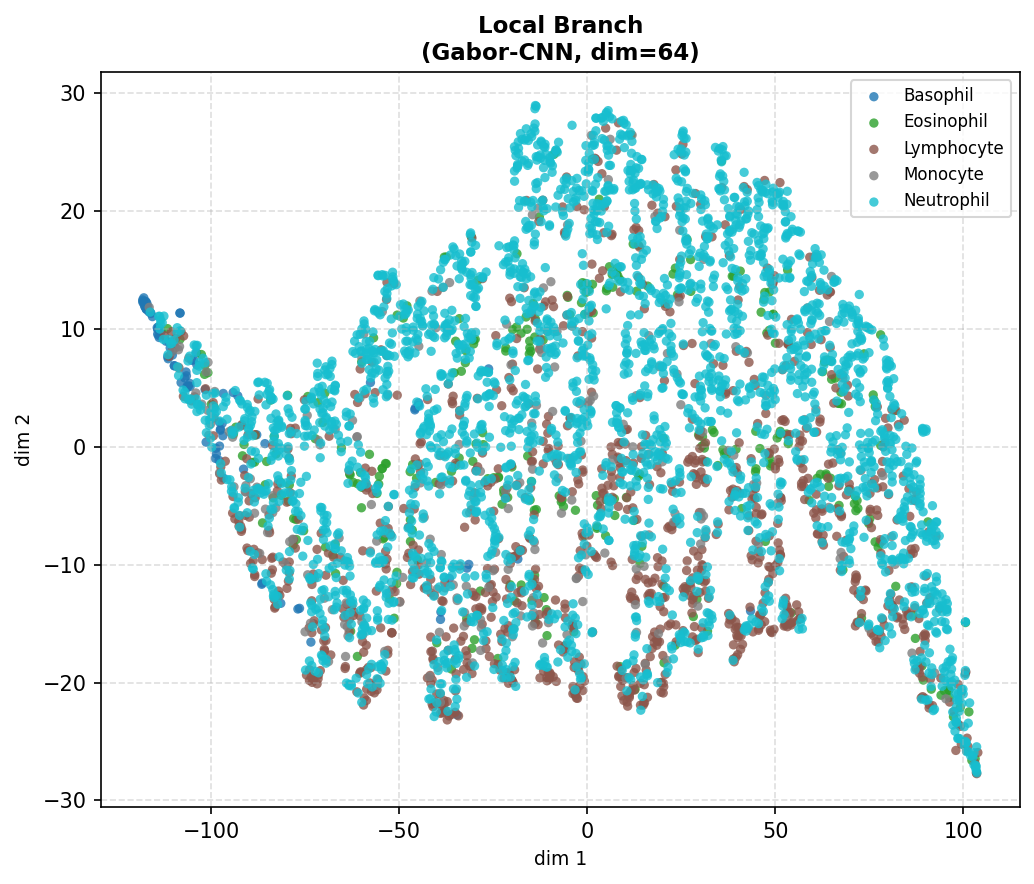
\includegraphics[width=0.5\linewidth]{tsne_local_branch.png} \\
\textbf{(g)}
\end{tabular}
&
\begin{tabular}{c}
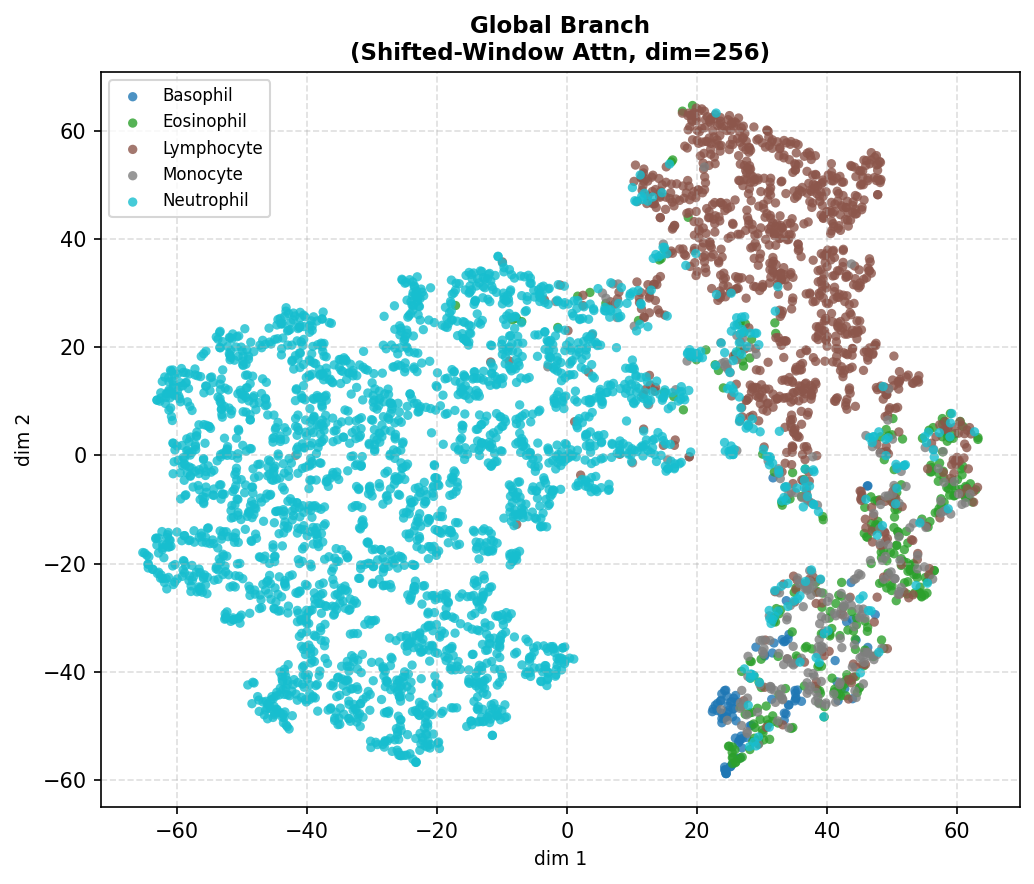
\includegraphics[width=0.5\linewidth]{tsne_global_branch.png} \\
\textbf{(h)}
\end{tabular}
&
\begin{tabular}{c}
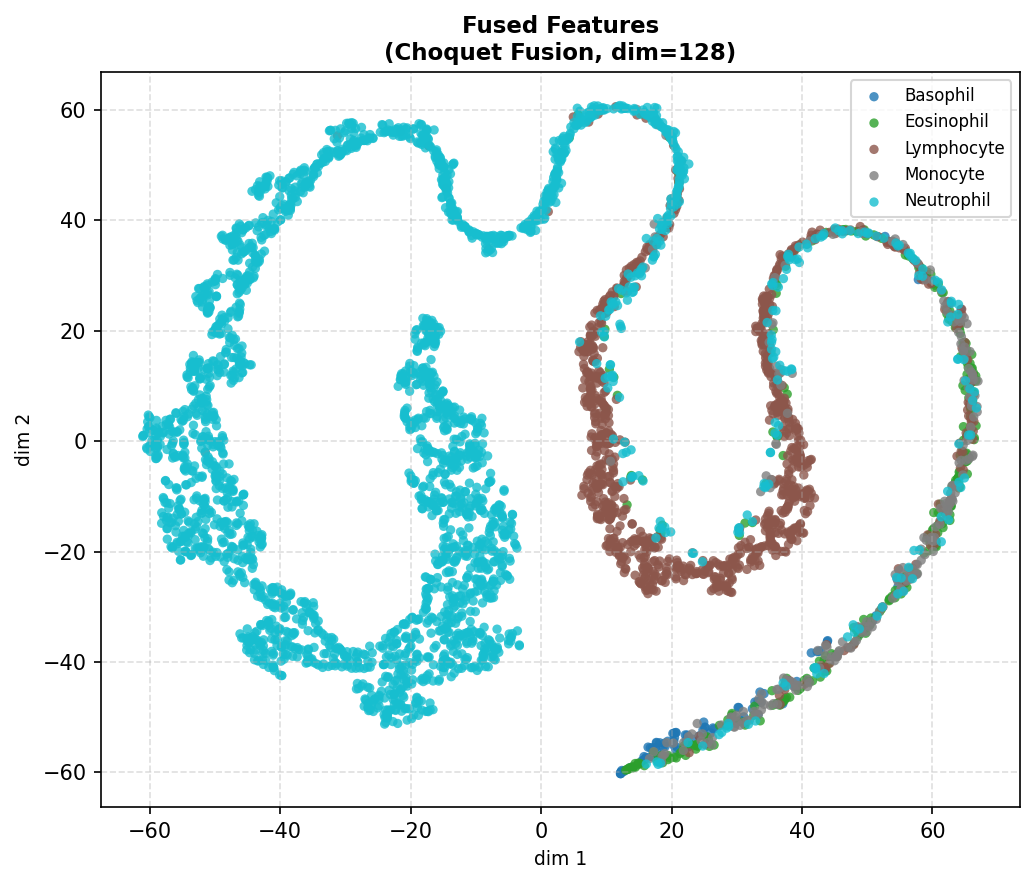
\includegraphics[width=0.5\linewidth]{tsne_fused.png} \\
\textbf{(i) Fusion}
\end{tabular}
\\ \hline

\end{tabular}%
}

\caption{t-SNE visualization of feature representations from local, global, and fused branches for BloodMNIST and WBC datasets.}
\label{tab:tsne_results}

\end{table*}


\begin{table*}[t]
\centering

\renewcommand{\arraystretch}{1.3}
\setlength{\tabcolsep}{6pt}

\resizebox{\linewidth}{!}{%
\begin{tabular}{|c|c|c|}
\hline

% -------- Row 1 --------
\begin{tabular}{c}
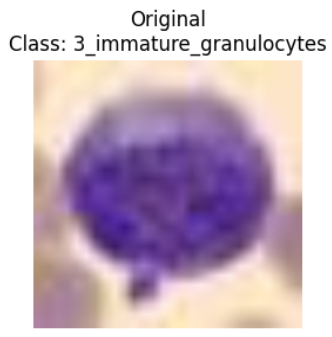
\includegraphics[width=0.4\linewidth]{gc1_granulo.png} \\
\textbf{(a)}
\end{tabular}
&
\begin{tabular}{c}
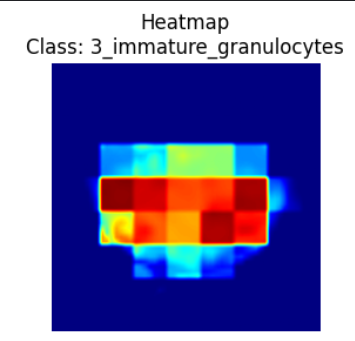
\includegraphics[width=0.4\linewidth]{gc1_granulo2.png} \\
\textbf{(b)}
\end{tabular}
&
\begin{tabular}{c}
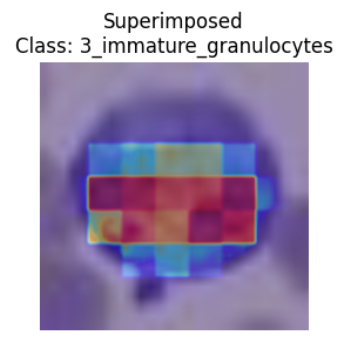
\includegraphics[width=0.4\linewidth]{gc1_granulo3.png} \\
\textbf{(c)}
\end{tabular}
\\ \hline

% -------- Row 2 --------
\begin{tabular}{c}
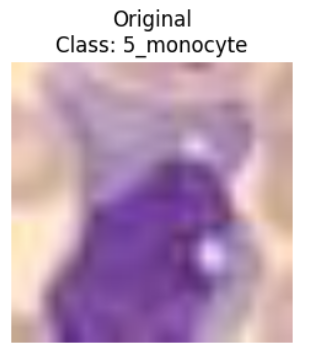
\includegraphics[width=0.4\linewidth]{gc1_monocyte.png} \\
\textbf{(d)}
\end{tabular}
&
\begin{tabular}{c}
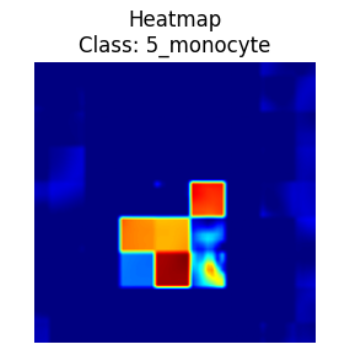
\includegraphics[width=0.4\linewidth]{gc1_monocyte2.png} \\
\textbf{(e)}
\end{tabular}
&
\begin{tabular}{c}
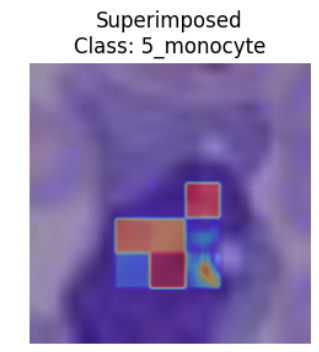
\includegraphics[width=0.4\linewidth]{gc1_monocyte3.png} \\
\textbf{(f)}
\end{tabular}
\\ \hline

% -------- Row 3 --------
\begin{tabular}{c}
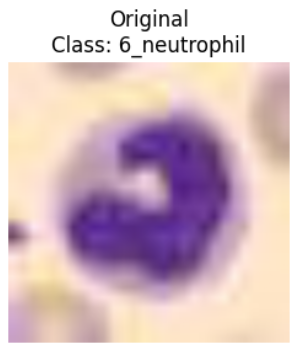
\includegraphics[width=0.4\linewidth]{gc1_neutrophil.png} \\
\textbf{(g)}
\end{tabular}
&
\begin{tabular}{c}
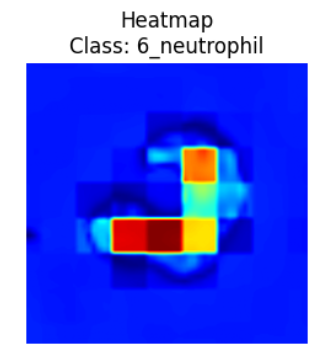
\includegraphics[width=0.4\linewidth]{gc1_neutrophil2.png} \\
\textbf{(h)}
\end{tabular}
&
\begin{tabular}{c}
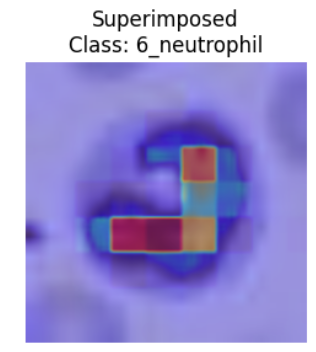
\includegraphics[width=0.4\linewidth]{gc1_neutrophil3.png} \\
\textbf{(i)}
\end{tabular}
\\ \hline

% -------- Row 4 --------
\begin{tabular}{c}
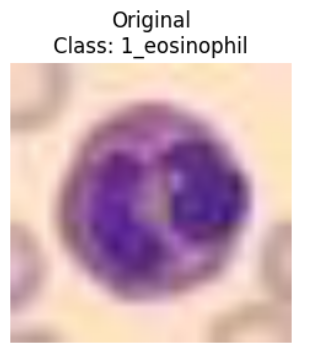
\includegraphics[width=0.4\linewidth]{gradcam1_eosinophil.png} \\
\textbf{(j)}
\end{tabular}
&
\begin{tabular}{c}
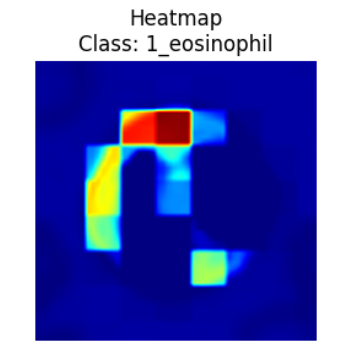
\includegraphics[width=0.5\linewidth]{gradcam1_eosinophil2.png} \\
\textbf{(k)}
\end{tabular}
&
\begin{tabular}{c}
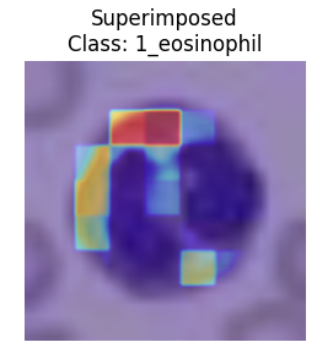
\includegraphics[width=0.4\linewidth]{gradcam1_eosinophil3.png} \\
\textbf{(l)}
\end{tabular}
\\ \hline

\end{tabular}
}

\caption{GradCAM visualization of local, global, and fused branches.}
\label{tab:gradcam_results}

\end{table*}

\begin{table*}[ht!]
\centering
\caption{Performance comparison on BloodMNIST and WBC datasets}
\label{tab:comparison}
\small
\setlength{\tabcolsep}{2pt}
\renewcommand{\arraystretch}{1.25}

\begin{tabular}{|p{3.35cm}|p{3.9cm}|p{2.9cm}|p{3.0cm}|p{2.9cm}|p{2.5cm}|}
\hline
\multicolumn{6}{|c|}{\textbf{Dataset: BloodMNIST}} \\ \hline
\textbf{Author} & \textbf{Model} & \textbf{Acc} & \textbf{Prec} & \textbf{Rec} & \textbf{F1} \\ \hline

Radhi et al. ~\cite{b16} & Quantum-EfficientNet & 0.96 & 0.95 & 0.96 & 0.95 \\ \hline

Shobiry et al. ~\cite{b17} & EfficientNetV2 + ANN & 0.76 & 0.75 & 0.72 & 0.73 \\ \hline

Shobiry et al. ~\cite{b17} & EfficientNetV2 + SVM & 0.77 & 0.75 & 0.74 & 0.74 \\ \hline

Patel et al. ~\cite{b18} & Swin + CNN & 0.95 & 0.94 & 0.95 & 0.95 \\ \hline

Radhi et al.~\cite{b16} & 6-Qubit VQC + EfficientNet-B0 & 0.96 & 0.95 & 0.95 & 0.96 \\ \hline

\textbf{Proposed} & Fuzzy fusion model & 0.98 & 0.96 & 0.98 & 0.97 \\ \hline

\multicolumn{6}{|c|}{\textbf{Dataset: WBC}} \\ \hline

Gao et al. ~\cite{b22} & MobileNetV2 & 0.97 & 0.96 & 0.95 & 0.96 \\ \hline

Toptaş et al. ~\cite{b20} & CNN Ensemble + SVM & 0.97 & 0.97 & 0.93 & 0.94 \\ \hline

Zou et al. ~\cite{b19} & ICAFF-MobileNetV2 & 0.90 & 0.90 & 0.90 & 0.90 \\ \hline

Baydilli et al. ~\cite{b21} & Capsule Network & 0.88 & 0.85 & 0.84 & 0.85 \\ \hline

Baydilli et al. ~\cite{b21} & Capsule Network(WBCaps) & 0.93 & 0.95 & 0.94 & 0.95 \\ \hline

\textbf{Proposed} & Fuzzy fusion model & 0.98 & 0.98 & 0.97 & 0.98 \\ \hline

\end{tabular}
\end{table*}



\FloatBarrier
\subsection{Ablation studies and Comparative Results}
The ablation studies are presented in \autoref{tab:ablation_bloodmnist} and \autoref{tab:ablation_wbc}. The comparative study with various state-of-the-art methods is reported in \autoref{tab:comparison}.

\begin{table}[ht!]
\centering
\caption{Performance of Different Model Variants on BloodMNIST dataset}
\label{tab:ablation_bloodmnist}
\begin{tabular}{|l|c|c|}
\hline
\textbf{Model Variant} & \textbf{Train Acc (\%)} & \textbf{Test Acc (\%)} \\ \hline

CNN with Gabor(local) & 91.85 & 89.01 \\ \hline
CNN with SWMHSA(Global) & 91.65 & 89.72 \\ \hline
Simple concatenation                  & 95.69 & 92.73 \\ \hline
Weighted average                  & 95.28 & 94.77 \\ \hline
Fused by only Minkowski distance           & 94.87 & 92.53 \\ \hline
Fused by only Parseval identity  & 94.36 & 92.88 \\ \hline
Proposed fusion  & 98.33 & 97.37 \\ \hline

\end{tabular}
\end{table}


\begin{table}[ht!]
\centering
\caption{Performance of Different Model Variants on WBC dataset}
\label{tab:ablation_wbc}
\begin{tabular}{|l|c|c|}
\hline
\textbf{Model Variant} & \textbf{Train Acc (\%)} & \textbf{Test Acc (\%)} \\ \hline

CNN with Gabor(local) & 91.33 & 90.25 \\ \hline
CNN with SWMHSA(Global) & 91.57 & 90.92 \\ \hline
Simple concatenation                  & 95.14 & 93.78 \\ \hline
Weighted average                  & 95.29 & 93.75 \\ \hline
Fused by only Minkowski distance           & 90.64 & 88.70 \\ \hline
Fused by only Parseval identity  & 94.35 & 93.06 \\ \hline
Proposed fusion  & 97.29 & 95.37 \\ \hline

\end{tabular}
\end{table}


\FloatBarrier
\subsection{Discussion}
The overall experimental evidence indicates that the proposed dual-branch formulation effectively combines complementary representations and yields a consistent gain over single-branch and naive fusion baselines. The local Gabor-CNN branch captures orientation-sensitive cellular micro-textures, while the shifted-window attention branch contributes wider contextual cues from nucleus--cytoplasm organization and surrounding morphology. This complementary behavior is reflected in the ablation results, where both individual branches remain near the low-90\% range, but the proposed fuzzy fusion produces a substantial jump in test performance on both BloodMNIST and WBC. Such a gain suggests that the improvement is not only due to increased parameterization, but also due to the interaction-aware fusion rule that modulates agreement and disagreement between branch-wise features.

The confusion matrices further support this interpretation. Most diagonal entries are strong, indicating high class-wise reliability, and the fused model reduces several off-diagonal confusions that remain visible in weaker baselines. In particular, classes with partially overlapping visual traits (e.g., granulocyte subtypes or morphologically close leukocyte categories) exhibit fewer mutual errors after fusion, implying better class boundary formation. At the same time, the residual off-diagonal pockets show that visually similar categories are still challenging under low-resolution or staining variability conditions. Therefore, the model is robust but not immune to fine-grained inter-class ambiguity, especially when diagnostic cues are subtle or partially occluded.

The Grad-CAM visualizations in \autoref{tab:gradcam_results} provide additional qualitative evidence of improved decision behavior. Compared with isolated local/global branches, the fused branch tends to concentrate activation around diagnostically meaningful regions (nuclear contour, chromatin-rich interior, and relevant cytoplasmic texture) with less irrelevant background emphasis. This indicates that fusion not only changes final logits but also improves where the model attends. A practical implication is better interpretability for medical screening workflows: when attention maps align with expected cellular structures, clinicians can more readily trust the model’s outputs. However, some samples still show diffuse or slightly shifted activations, revealing that saliency stability is not yet uniform across all classes and image conditions.

The t-SNE projections in \autoref{tab:tsne_results} are consistent with the quantitative and Grad-CAM findings. Local and global embeddings individually show partial clustering with noticeable overlaps, while fused embeddings demonstrate tighter intra-class grouping and better inter-class separation. This geometric consolidation aligns with the proposed Choquet--Minkowski--Parseval mechanism, where agreement-aware weighting and distance-sensitive modulation help suppress conflicting branch evidence. Better manifold separation can explain the improved generalization seen in test metrics. Nevertheless, some class neighborhoods remain close in the fused space, suggesting that separability is improved but not fully saturated.

From a strengths perspective, the model offers: (i) strong cross-dataset performance, (ii) clear ablation-backed contribution from each component, (iii) improved explainability through Grad-CAM behavior, and (iv) better feature geometry indicated by t-SNE structure. These attributes make the method promising for practical blood-cell analysis pipelines where both accuracy and interpretability matter. From a limitations perspective, several drawbacks remain. First, the approach introduces additional design complexity compared with simpler end-to-end backbones, including multiple branches and a non-trivial fusion rule. Second, although errors are reduced, confusion among morphologically similar classes persists, indicating limited robustness under severe class overlap. Third, t-SNE and saliency analyses are supportive but still post-hoc; they do not guarantee causal interpretability. Finally, performance has been validated on two datasets, and broader multi-center/domain-shift evaluation is still required for stronger clinical transfer claims.

Overall, the findings suggest that the proposed fusion strategy is a meaningful step beyond standard concatenation/averaging and provides a better balance between discriminative power and interpretability. The most promising future direction is to combine this fusion framework with stronger domain adaptation, stain normalization, and uncertainty calibration so that residual hard cases can be handled more reliably in real-world deployment.

 \section{Conclusion}
In this paper, we proposed a dual-branch architecture that integrates a Gabor-based CNN for capturing fine-grained local features and a CNN with shifted window attention to model global contextual dependencies. The complementary representations from both branches are fused using a novel Choquet integral-inspired fuzzy fusion mechanism enhanced by Minkowski distance and Parseval-based energy alignment, enabling adaptive and uncertainty-aware feature aggregation. The proposed model demonstrates superior performance on both BloodMNIST and WBC datasets, outperforming several contemporary approaches and validating the effectiveness of combining local–global feature learning with advanced fusion strategies.

Despite these promising results, certain misclassifications still persist, particularly among visually similar cell types, indicating scope for further improvement. Future work will focus on exploring more advanced attention-driven fusion mechanisms, incorporating domain-specific preprocessing techniques, and evaluating the model on additional large-scale medical datasets to further enhance robustness and generalization capability.

\FloatBarrier
\begin{thebibliography}{00}
\bibitem{b1}
D. Gabor,
``Theory of Communication,''
Journal of the Institution of Electrical Engineers (JIEE), Vol. 93, Part III, pp. 429--457, 1946.

\bibitem{b2}
A. K. Jain and F. Farrokhnia,
``Unsupervised Texture Segmentation Using Gabor Filters,''
IEEE Transactions on Pattern Analysis and Machine Intelligence (PAMI),
Vol. 13, No. 11, pp. 1167--1186, 1991.

\bibitem{b3}
T. S. Lee,
``Image Representation Using 2D Gabor Wavelets,''
IEEE Transactions on Pattern Analysis and Machine Intelligence (PAMI),
Vol. 18, No. 10, pp. 959--971, 1996.

\bibitem{b4}
A. Vaswani, N. Shazeer, N. Parmar, J. Uszkoreit, L. Jones, A. N. Gomez, 
L. Kaiser and I. Polosukhin,
``Attention Is All You Need,''
Advances in Neural Information Processing Systems (NeurIPS),
pp. 5998--6008, 2017.

\bibitem{b5}
Z. Liu, Y. Lin, Y. Cao, H. Hu, Y. Wei, Z. Zhang, S. Lin and B. Guo,
``Swin Transformer: Hierarchical Vision Transformer Using Shifted Windows,''
Proceedings of the IEEE/CVF International Conference on Computer Vision (ICCV),
pp. 10012--10022, 2021.

\bibitem{b6}
G. Choquet,
``Theory of Capacities,''
Annales de l’Institut Fourier,
Vol. 5, pp. 131--295, 1953--1954.

\bibitem{b7}
M. Grabisch, T. Murofushi and M. Sugeno,
``Fuzzy Measures and Integrals: Theory and Applications,''
Studies in Fuzziness and Soft Computing, Springer,
Vol. 40, 2000.

\bibitem{b8}
M. Grabisch, J.-L. Marichal, R. Mesiar and E. Pap,
``Aggregation Functions,''
Encyclopedia of Mathematics and its Applications, Cambridge University Press,
Vol. 127, 2009.

\bibitem{b9} 
H. Minkowski,
``Beiträge zur Theorie der konvexen Körper,''
Nachrichten von der Gesellschaft der Wissenschaften zu Göttingen, 
Mathematisch-Physikalische Klasse, pp. 198--219, 1896.

\bibitem{b10}
X. Zhu and D. L. Smith,
``Comparison of Distance Measures in Spatial Analytical Modeling,''
Proceedings of the International Conference on Geographic Information Science (GIScience),
pp. 1--12, 2004.



\bibitem{b11}
M.-A. Parseval des Chênes,
``Über Fourierreihen,''
Mémoires présentés à l’Institut des Sciences, Lettres et Arts, 
pp. 638--648, 1799.


\bibitem{b12}
A.-L. Cauchy,
``Cours d’Analyse de l’École Royale Polytechnique,''
Imprimerie Royale, Paris, 1821.

\bibitem{b13}
H. A. Schwarz,
``Gesammelte mathematische Abhandlungen,''
Springer, Berlin, 1890.

\bibitem{b14}
T. Tanimoto,
``An Elementary Mathematical Theory of Classification and Prediction,''
IBM Internal Report, 1958.

\bibitem{b15}
A. O. Boudraa, J. C. Cexus and Z. Saidi,
``An Energy-Based Similarity Measure for Time Series,''
IEEE International Conference on Acoustics, Speech, and Signal Processing (ICASSP),
pp. 1973--1976, 2008.
2023.

\bibitem{b16}
E. A. Radhi, M. A. Mohammed, F. Eid and I. de la Torre Díez,
``Efficient Blood Cell Classification Using a Hybrid Variational Quantum Circuit–EfficientNet Model on BloodMNIST,''
Journal of Artificial Intelligence and Medical Applications (JAIMA),
Vol. 1, No. 1, 2023, doi: 10.65511/jaima.v1i1.734.

\bibitem{b17}
A. K. F. Shobiry and R. Puspitasari,
``Hybrid Feature Benchmark for Blood Cell Classification Using ResNet50 and EfficientNetV2 Features with SVM and ANN Classifiers via Unsupervised Segmentation,''
International Journal of Artificial Intelligence and Machine Intelligence (IJAIMI),
Vol. 3, No. 2, 2024, doi: 10.56705/ijaimi.v3i2.364.

\bibitem{b18}
T. Patel, H. El-Sayed, M. K. Sarker, D. Duong and B. D. Solomon,
``Training Swin Transformer-Based GAN for High-Resolution Blood Cell Imaging with Limited Data,''
Computational Science and Computational Intelligence (CSCI 2024),
Communications in Computer and Information Science (CCIS), Vol. 2511,
pp. 161--176, Springer, 2025. 

\bibitem{b19}
Y. Zou, L. Wu, C. Zuo, L. Chen, B. Zhou and H. Zhang,
``White Blood Cell Classification Network Using MobileNetV2 with Multiscale Feature Extraction Module and Attention Mechanism,''
Biomedical Signal Processing and Control,
Vol. 91, 2024, doi: 10.1016/j.bspc.2024.106820. 

\bibitem{b20}
B. Toptaş, M. K. Öztürk and H. T. Kahraman,
``Classification of White Blood Cells Using CNN Ensemble and Support Vector Machine,''
Biomedical Signal Processing and Control,
Vol. 66, 2021.

\bibitem{b21}
Y. Y. Baydilli and Ü. Atila,
``Classification of White Blood Cells Using Capsule Networks,''
Computerized Medical Imaging and Graphics,
Vol. 80, 2020, doi: 10.1016/j.compmedimag.2020.101699.

\bibitem{b22}
W. Gao, L. Lan and X. Fan,
``DaNet: Domain-Adaptive White Blood Cell Classification Through Synthetic Augmentation and Cross-Domain Feature Alignment,''
Array,
2025, doi: 10.1016/j.array.2025.100416.

\bibitem{b23}
H. Fırat,
``Classification of Microscopic Peripheral Blood Cell Images Using Multibranch Lightweight CNN-Based Model,''
Neural Computing and Applications,
Vol. 36, 2024, doi: 10.1007/s00521-023-09158-9.

\bibitem{b24}
R. Girdhar, A. Gupta and S. Gupta,
``White Blood Cell Classification Using CNN-Based Framework on BCCD Dataset,''
Proceedings of the International Conference on Computing, Communication and Automation (ICCCA),
pp. 1--6, 2019.

\bibitem{b25}
M. Bećirović, A. Kurtović, N. Smajlović, M. Kapo and A. Akagić,
``Performance Comparison of Medical Image Classification Systems Using TensorFlow Keras, PyTorch, and JAX,''
arXiv preprint arXiv:2507.14587, 2025.

\bibitem{b26}
P. Payne, R. V. Romould, J. Mondal, R. Chatterjee, and M. K. Gourisaria,
``Beyond Microscope: Advances in Technology for Detection of Cervical Cancer,''
in \textit{Proc. ICPR 2024, LNCS 15614}, Springer, 2025, pp. 180--193,
doi: $10.1007/978-3-031-87657-8_13$.


\bibitem{b27}
T. Sood, P. Khandnor, and R. Bhatia,
``Enhancing Pap Smear Image Classification: Integrating Transfer Learning and Attention Mechanisms for Improved Detection of Cervical Abnormalities,''
\textit{Biomedical Physics \& Engineering Express}, vol. 10, 2024, Art. no. 065031.
doi: 10.1088/2057-1976/ad7bc0.


\bibitem{b28}
S. Singh, C. Sahu, P. Singh, A. Mishra, S. K. Mishra, and P. K. Patnaik,
``Refining Cell Classification for Cervical Cancer Detection Using an Improved High Dimensional Feature Fusion Approach,''
\textit{Medical Engineering \& Physics}, vol. 146, p. 104445, 2025.
doi: 10.1016/j.medengphy.2025.104445.


\bibitem{b29}
T. A. Emon, M. M. Shakil, N. Tahsin, S. Sarkar, N. T. Progga, and Z. Jiyad,
``MultiArchFusionV16Ensemble: A Novel Neural Network Based Ensemble Model for Enhanced Cervical Cancer Detection,''
in \textit{Proc. 3rd Int. Conf. Computing Advancements (ICCA)}, ACM, 2024.
doi: 10.1145/3723178.3723316.


\bibitem{b30}
D. Julie, N. P., P. K., and S. Devi,
``Enhancing Cervical Cancer Diagnosis using Deep Learning based CAD Systems,''
in \textit{Proc. 5th Int. Conf. Pervasive Computing and Social Networking (ICPCSN)}, IEEE, 2025.
doi: 10.1109/ICPCSN65854.2025.11035806.


\bibitem{b31}
A. Khowaja, B. Zou, and X. Kui,
``Enhancing Cervical Cancer Diagnosis: Integrated Attention-Transformer System with Weakly Supervised Learning,''
\textit{Image and Vision Computing}, vol. 149, p. 105193, 2024.
doi: 10.1016/j.imavis.2024.105193.
\end{thebibliography}

\end{document}